%%%%%%%%%%%%%%%%%%%%%%%%%%%%%%%%%%%%%%%%%
% baposter Landscape Poster
% LaTeX Template
% Version 1.0 (11/06/13)
%
% baposter Class Created by:
% Brian Amberg (baposter@brian-amberg.de)
%
% This template has been downloaded from:
% http://www.LaTeXTemplates.com
%
% License:
% CC BY-NC-SA 3.0 (http://creativecommons.org/licenses/by-nc-sa/3.0/)
%
%%%%%%%%%%%%%%%%%%%%%%%%%%%%%%%%%%%%%%%%%

%----------------------------------------------------------------------------------------
%	PACKAGES AND OTHER DOCUMENT CONFIGURATIONS
%----------------------------------------------------------------------------------------

\documentclass[landscape,a0paper,fontscale=0.285]{baposter} % Adjust the font scale/size here

\usepackage{graphicx} % Required for including images
\graphicspath{{figures/}} % Directory in which figures are stored

\usepackage{amsmath} % For typesetting math
\usepackage{amssymb} % Adds new symbols to be used in math mode
\usepackage{geometry}
\usepackage{booktabs} % Top and bottom rules for tables
\usepackage{enumitem} % Used to reduce itemize/enumerate spacing
%\usepackage{palatino} % Use the Palatino font
\usepackage{graphicx}
\usepackage{subfig}
\usepackage{caption}
\usepackage{booktabs}
\usepackage[font=small,labelfont=bf]{caption} % Required for specifying captions to tables and figures

%COLORS
\definecolor{bordercol}{RGB}{40,40,40} % Border color of content boxes
\definecolor{headercol1}{RGB}{186,215,230} % Background color for the header in the content boxes (left side)
\definecolor{headercol2}{RGB}{80,80,80} % Background color for the header in the content boxes (right side)
\definecolor{headerfontcol}{RGB}{0,0,0} % Text color for the header text in the content boxes
\definecolor{boxcolor}{RGB}{186,215,230} % Background color for the content in the content boxes
\definecolor{purple}{RGB}{91, 59, 140}


\definecolor{bleunuit}{RGB}{0,38,84}
\definecolor{cyan}{RGB}{96,175,221}
\definecolor{bleugris}{RGB}{155,175,196}
\usepackage{multicol} % Required for multiple columns
\setlength{\columnsep}{0.5em} % Slightly increase the space between columns
\setlength{\columnseprule}{0mm} % No horizontal rule between columns
\usepackage{float}
\usepackage{tikz} % Required for flow chart
\usetikzlibrary{shapes,arrows}
\usetikzlibrary{positioning}
\tikzstyle{block} = [rectangle, draw, rounded corners]
\tikzstyle{line} = [draw, -latex']

\newcommand{\compresslist}{ % Define a command to reduce spacing within itemize/enumerate environments, this is used right after \begin{itemize} or \begin{enumerate}
\setlength{\itemsep}{1pt}
\setlength{\parskip}{0pt}
\setlength{\parsep}{0pt}
}

%Lenght Between figure and caption
\setlength{\abovecaptionskip}{15pt plus 0pt minus 2pt} 
\setlength{\tabcolsep}{2.5pt}
%Header Height
\setlength{\headsep}{5mm}
\setlength{\topskip}{50mm}
%\setlength{\oddsidemargin}{0mm}
%\setlength{\textwidth}{184.3mm}
%\setlength{\columnsep}{6.3mm}
%\setlength{\marginparsep}{0mm}
%\setlength{\marginparwidth}{0mm}
%\setlength{\textheight}{265.2mm}
\definecolor{lightblue}{rgb}{0.145,0.6666,1} % Defines the color used for content box headers
\begin{document}
	
	\tikzstyle{block} = [draw, fill=white, rectangle, 
	minimum height=2.5em, minimum width=6em]
	\tikzstyle{sum} = [draw, fill=white, circle, node distance=2cm]
	\tikzstyle{input} = [coordinate]
	\tikzstyle{output} = [coordinate]
	\tikzstyle{pinstyle} = [pin edge={to-,thin,black}]
	%Here I put the title, first slide	
%	\setpostertemplate{itemize items}[circle]
%	\setbeamertemplate{enumerate items}[circle]

\begin{poster}
{
headerborder=closed, % Adds a border around the header of content boxes
colspacing=0.1em, % Column spacing
bgColorOne=white, % Background color for the gradient on the left side of the poster
bgColorTwo=white, % Background color for the gradient on the right side of the poster
borderColor=lightgray, % Border color
headerColorOne=purple, % Background color for the header in the content boxes (left side)
headerColorTwo=purple, % Background color for the header in the content boxes (right side)
headerFontColor=white, % Text color for the header text in the content boxes
boxColorOne=white, % Background color of the content boxes
textborder=roundedleft, % Format of the border around content boxes, can be: none, bars, coils, triangles, rectangle, rounded, roundedsmall, roundedright or faded
eyecatcher=false, % Set to false for ignoring the left logo in the title and move the title left
headerheight=0.1\textheight, % Height of the header
headershape=roundedright, % Specify the rounded corner in the content box headers, can be: rectangle, small-rounded, roundedright, roundedleft or rounded
headerfont=\large\bf\textsc, % Large, bold and sans serif font in the headers of content boxes
%textfont={\setlength{\parindent}{1.5em}}, % Uncomment for paragraph indentation
headerheight=2.2cm,
columns=4,
linewidth=0.1pt % Width of the border lines around content boxes
}
%----------------------------------------------------------------------------------------
%	TITLE SECTION 
%----------------------------------------------------------------------------------------

{{\color{bleunuit}\LARGE\bf\textsc{The Economics of Shotgun Marriage}\vspace{0.3em}}} % Poster title
{{\color{bleunuit}\LARGE{Egor Kozlov  \hspace{2pt}---\hspace{2pt} Northwestern University, \textbf{egorkozlov2020@u.northwestern.edu}}}} % Author names and institution
%----------------------------------------------------------------------------------------
%	Motivation
%----------------------------------------------------------------------------------------

\headerbox{1. Shotgun Marriages Are Widespread and Do Not End Well}{name=motivation,column=0,row=-0.015,span=2}{
	\begin{minipage}{0.65\linewidth}
	\footnotesize
	\begin{itemize}
\item Many people marry shortly after a baby appears
\begin{itemize}
\item Shotgun marriage = first child before or at the year of marriage
\item $\sim10\%$ marry while being pregnant
\item Even more marry after their first birth
\item Not just teenage pregnancies, many among 25+ 
\item I view these pregnancies as unplanned yet not exogenous
\end{itemize}
\item People who had a shotgun marriage divorce more in the data 
\begin{itemize}
\item A lot more for college grads, a bit more for high school grads
\end{itemize}
\item Understanding why helps to understand the value of marriage
\item Questions:
\begin{itemize}
\item What is the aggregate role of unplanned pregnancies?
\item What causes people to enter such marriages?
\item Why they perform worse?
\end{itemize}
\end{itemize}
	\end{minipage}
	\hfill
	\begin{minipage}{0.35\linewidth}	
			\begin{center}
			\includegraphics[scale=0.3]{graph_dt_poster.eps}
			 \includegraphics[scale=0.3]{share_kj_poster.eps}
			 \end{center}
    \end{minipage}
   }


\headerbox{2. Model Is Required Here}{name=rq,column=2,row=-0.015,bottomaligned=motivation,span=1}{
	\vspace*{-0.4mm}
{\footnotesize
\begin{itemize}
\item Quantify empirical difference of marriage performance by the timing of childbirth:
\vspace{-1mm}
\begin{itemize}
\item Main sample: ACS 2009--2016, women  21--40 with one marriage (limited marriage history)
\vspace{-1mm}
\item Robustness (full history): SIPP, NSFG, NSFH
%, cross-sectional regressions and duration models
\end{itemize}
\item Estimate a lifecycle model matching this difference
\vspace{-2mm}
\begin{itemize}
\item limited commitment: marriage and divorce
\item savings and heterogeneous productivity
\item fertility choice and shocks
\end{itemize}
\vspace{-2mm}
\item Use the model to study:
\vspace{-1mm}
\begin{itemize}
\item aggregate impact of unplanned childbirths 
\item importance of fertility for marriage
\item difference between education groups
\item policy counterfactuals
\end{itemize}
\end{itemize}
}
}



%----------------------------------------------------------------------------------------
%	Methodology
%---------------------------------------------------------------------------------------
\headerbox{3. Bad Performance Data Facts}{name=meth,column=3,bottomaligned=motivation,row=-0.015,span=1}{
	\vspace*{-0.4mm}
	\footnotesize
	\[\Delta T = \text{Age 1st birth} - \text{Age 1st marriage}.\]
	\begin{itemize}
	\item Kids First (KF): $\Delta T \in \{-5,...,0\}$
	\item Marriage First (MF): $\Delta T \in \{1,...,10\}$
	\end{itemize}
	\vspace{-1em}
	\begin{center}
	\begin{tabular}{|l|c|c|c|c||c|}\hline
	\multicolumn{6}{|c|}{ \textit{ACS: women, married once and have kids}, 21--40}\\\hline
	& \multicolumn{2}{|c|}{\% divorced} & ratio & ratio & \% of  \\ 
	& \textbf{MF} & \textbf{KF} &  (raw) &   (reg)  & KF\\\hline
	Everyone  & 10.1 & 18.0 & \textbf{1.8} & 1.6 & 22.8 \\
	High School & 13.9 &  17.2 & \textbf{1.2} & 1.6 &  33.3 \\
	College & 5.3  & 14.7 & \textbf{2.8}  & 1.7 &  9.5\\
	First birth 25+ & 7.2 & 10.8 & \textbf{1.5} & 1.6 & 8.6 \\\hline
	\multicolumn{6}{|p{0.8\linewidth}|}{\scriptsize These are cross-sectional shares of divorced. ``Divroced'' is being divorced at the moment of the survey. ``Reg'' refers to regression-adjusted ratio with controls: age, age at 1st marriage, age at 1st birth, education, race, state,  ACS year, number of children}\\\hline
	\end{tabular}
	\end{center}
	\vspace{-0.5em}
	\textbf{Main conclusion:} \textit{women who experience a shotgun marriage experience more divorces in all subsamples.}
}


%----------------------------------------------------------------------------------------
%	Data
%---------------------------------------------------------------------------------------
\headerbox{4. The Results Are Stable}{name=data,column=0,row=0.355,span=1}{
\footnotesize
Very similar conclusions are obtained by
	\begin{itemize}
	\item ACS (large samples but incomplete history):
	\vspace{-0.5em}
	\begin{itemize}
	\item Controlling for income (if full-time working)\vspace{-0.25em}
	\item Comparing only marriages of the same duration\vspace{-0.25em}
	\end{itemize}
	\vspace{-0.5em}
	\item SIPP: smaller sample with better marital history (not just married once)\vspace{-0.25em}
	\item NSFH and NSFG: allow to run duration analysis\vspace{-0.5em}
	\begin{itemize}
	\item rel hazards of divorce $\approx$ cross-sectional ratios\vspace{-0.25em}
	\item $\Delta T$ in months, exclusion of step children\vspace{-0.25em}
	\end{itemize}
	\end{itemize}
	
	
Additional insights:
	\begin{itemize}
	\item Marriages with $\Delta T = 0$ have the worst performance
	\item Divorces are concentrated around child's age 5--10
	\item Children in KF couples repeat grades more often
	\vspace{2em}
	\end{itemize}
	}
%
%\headerbox{4. Model: Summary}{name=data,column=0,row=0.355,span=1}{
%\footnotesize
%\begin{itemize}
%\item Key features:
%\vspace{-0.5em}
%\begin{itemize}
%\item Males $m$, females $f$; singles $s$, couples $c$
%\item Assets ($a$) and productivity ($z^f$, $z^m$), ``love'' $\psi$
%\item Endogenous marriage and divorce, $p^{\text{meet}}(\text{Age})$
%\item Unplanned pregnancy can happen \textbf{when potential partners meet}: $p^{\text{unplanned}}(\text{Age})$
%\item \textbf{Married couples}: optimal fertility (1 child)
%\end{itemize}
%\item Unplanned pregnancy triggers marriage because of:
%\begin{itemize}
%\item Large childcare expenditures need to be shared
%\item Marriage prospects of single mothers are worse
%\end{itemize}
%\textbf{Result:} preg shock $\Rightarrow$ couples with lower $\psi$ marry
%\end{itemize}
%}

\headerbox{5. Model: Limited Commitment + Optimal Fertility In Couple + Pregnancy Shocks When Meet}{name=theory,column=1,row=0.355,span=3}{
\vspace{-0.25cm}
\hspace{-0.75cm}
\begin{tabular}{c c c c}
\begin{minipage}{0.3\linewidth}
\footnotesize
\begin{itemize}
\item Key features:
\vspace{-0.75em}
\begin{itemize}
\item Males $m$, females $f$; singles $s$, couples $c$\vspace{-0.25em}
\item Heterogeneous earnings $W$ and savings $a$\vspace{-0.25em}
\item Couple-specific $\psi$ --- relationship quality\vspace{-0.25em}
\item Random but assortative mating\vspace{-0.25em}
\item Endogenous marriage and divorce\vspace{-0.25em}
\item Unplanned pregnancy can happen \textbf{when potential partners meet}\vspace{-0.25em}
\item \textbf{Married couples} have optimal fertility\vspace{-0.25em}
\end{itemize}
\item Unplanned pregnancy $\Rightarrow$ low-quality marriage:
\begin{itemize}
\item Childcare expenditures need to be shared
\item Marriage prospects of single mothers drop
\end{itemize}
\textbf{Result:} preg shock $\Rightarrow$ couples with lower $\psi$ marry
\end{itemize}
\end{minipage}
&
\hspace{-0.25cm}
\begin{minipage}{0.27\linewidth}
\vspace{0.0cm}
\begin{center}
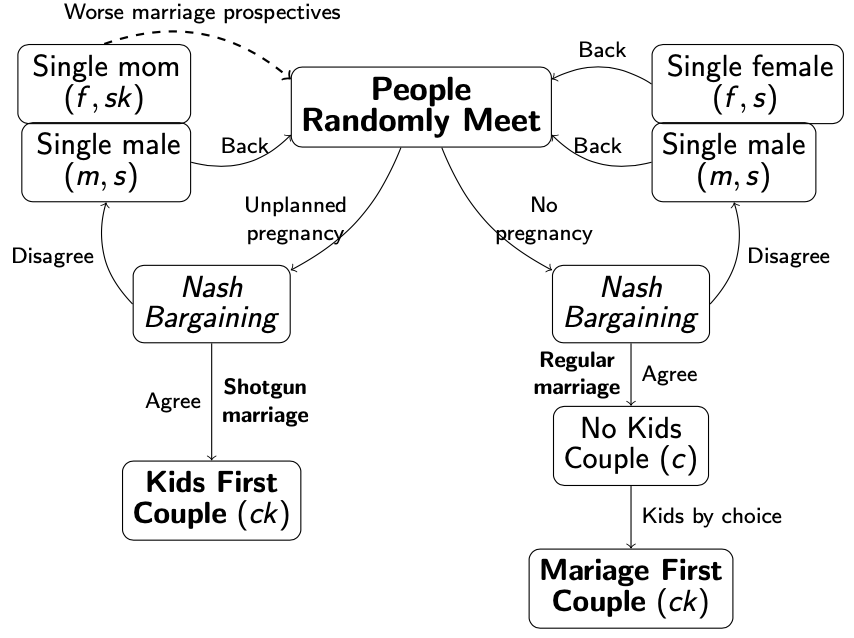
\includegraphics[scale=0.35]{scheme.png}
\end{center}
\vspace{-2em}
{\scriptsize \hspace{0.4cm} Marry if $\exists \theta$ s.t.:\vspace{-0.25em}
\begin{itemize}
\item { $\scriptstyle \text{No shock: } V^{f,c}(\theta) \geq V^{f,s} \text{ and } V^{m,c}(\theta) \geq V^{m,s}$}\vspace{-0.4em}
\item { $\scriptstyle \text{Shock: } V^{f,ck}(\theta) \geq V^{f,sk} \text{ and } V^{m,ck}(\theta) \geq V^{m,s}$}\vspace{-0.4em}
\item {$\scriptstyle \text{Single mom} \, = \, \text{Shock, but } V^{m,ck}(\theta) \geq V^{m,s} - \phi^r$}
\end{itemize}
}
\end{minipage}

&
\hspace{-2em}
\begin{minipage}{0.225\linewidth}
{\footnotesize
\vspace{0.3em}
\hspace{2em}\textbf{Value Functions:}
\vspace{-0.5em}
\[\hspace{-2em}m \text{ --- marriage }, \ \ \ d  \text{ --- divorce}\]
\vspace{-2em}
\begin{align*} \scriptsize
& V^{f,s}_t =  u(c_f) + \beta\mathbb{E}_t \big[(1-p^{\text{meet}}_t)\cdot V^{f,s}_{t+1}  \\ + & p^{\text{meet}}_t \big\{ p^{\text{preg}}_t (m_{t+1} V^{f,ck}_{t+1} + (1-m_{t+1})V^{f,sk}_{t+1})  
\\  +  &  (1-p^{\text{preg}}_t) (m_{t+1} V^{f,c}_{t+1} + (1-m_{t+1})V^{f,s}_{t+1})  \big\} \big].
\end{align*}
\vspace{-0.5cm}
\begin{align*} \scriptsize
& V^c_t =  \theta^f \cdot u(c_f) + \theta^m \cdot u(c_m) + \psi \\
+ & \beta\mathbb{E}_t \big[\max\{V^{ck}_{t+1},V^{c}_{t+1}\}\cdot (1-d_{t+1}) 
\\ +  & d_{t+1} \cdot(\theta^f\cdot V^{f,s}_{t+1} + \theta^m\cdot V^{m,s}_{t+1})\big].
\end{align*}
\vspace{-0.5cm}
\begin{align*} \scriptsize & V^{c,k}_t =  \theta^f \cdot u(c_f) + \theta^m \cdot u(c_m) + \psi  \\
+ & u^{\text{kid}}(Q) +  \beta\mathbb{E}_t \big[V^{ck}_{t+1}\cdot (1-d_{t+1}) 
\\ +  & d_{t+1} \cdot(\theta^f\cdot V^{f,sk}_{t+1} + \theta^m\cdot V^{m,s}_{t+1})\big].
\end{align*}
%\begin{itemize}
%\item $\theta$ stays constant if p.c. don't bind
%\item $\theta$ may be renegotiated
%\item If no agreeable $\theta$ $\Rightarrow$ divorce
%\item Low $\psi$ $\Rightarrow$ more likely to divorce
%\end{itemize}
%\hspace{2em}\textbf{Upon Divorce}:
%\begin{itemize}
%\item Only moms pay childcare
%\item Fathers lose access to their kids
%\item Single moms remarry $\Rightarrow$ utility loss of $\phi^r$ for their new partner
%\end{itemize}
}
\end{minipage}
&
\hspace{-2em}
\begin{minipage}{0.225\linewidth}
\vspace{-0.5cm}
{\footnotesize
%\textbf{Notation:} $c$ --- consumption, $\theta$ --- Pareto weight, $\psi$ --- common love shock, $x$ --- child expenditures, $l$ --- labor supply, $t$ --- age.
\begin{itemize}
%\item Child's consumption: $Q = F(x,1-l^f)$
\item S.t. participation constraints:
\vspace{-0.5em}
\[\scriptstyle V^{f,c\bullet}_t \geq V^{f,\text{divorce}}_t, \ V^{m,c\bullet}_t \geq V^{m,\text{divorce}}_t,\]
\vspace{-2em}
\item Violated $\Rightarrow$ renegotiation or divorce
\item Childcare ($x$ --- money, $l^f$ --- labor)
\vspace{-1.0em}
\[\scriptstyle Q = f(x,1-l^f), \ \ Q \geq \bar{Q} \ (\text{subsistence})\]
\vspace{-1.5em}
\item Budget ($\rho>1$ --- returns to scale): 
\vspace{-0.75em}
\[\scriptstyle (c_f^{\rho} + c_m^{\rho})^{\frac1{\rho}} + a' + x = R\cdot a + l^f \cdot W^f_t + W^m_t\]
\[\scriptstyle W^i_t= \exp\left\{z_i + \text{Trend}_{i,t}\right\}\]
\vspace{-1.75em}
\item Shocks: $\scriptstyle z_m' = z_m + \varepsilon^{z}_m$, $\scriptstyle \psi' = \psi + \varepsilon^{\psi}$ 
\item Female productivity can depreciate:
\vspace{-0.75em}
\[\scriptstyle z_f' = z_f -  \text{{\boldmath $\delta (l^f)$}} + \varepsilon^{z}_f.\]
\item Female stays with the child and do not get any child support if divorced
\end{itemize}
}
\end{minipage}
\end{tabular}
}



%----------------------------------------------------------------------------------------
%	Estimation
%---------------------------------------------------------------------------------------
\headerbox{6. Estimation: MSM}{name=estimation,column=0,span=1,row=0.662}{
\footnotesize
	 \begin{itemize}
	 \item Two samples: college and high school graduates
	 \item Income process and trend: match ACS
	 \item I fix externally:\vspace{-0.5em}
	 \begin{itemize}
	 \item Couple's returns to scale $\rho$ (Voena, 2015)\vspace{-0.25em}
	 \item Skill depreciation (Adda et al, 2017)\vspace{-0.25em}
	 \item Substitutability between $l$ and $x$ (Sommer, 2016)\vspace{-0.25em}
	 \item Standard $\beta = R^{-1} = 0.98$ \vspace{-0.25em}
	 \end{itemize}
	 \item Method of Simulated Moments picks parameters for:\vspace{-0.5em}
	 \begin{itemize}
	 \item Transition probabilities: $p^{\text{preg}}_t$, $p^{\text{meet}}_t$\vspace{-0.25em}
	 \item Choice parameters: $u^{\text{kid}}(Q)$, $Q(x,1-l_f)$, $\bar{Q}$\vspace{-0.25em}
	 \item Love shock distribution: $\sigma(\varepsilon^\psi)$, $\sigma(\psi_0)$.\vspace{-0.25em}
	 \item Drop in marriage prospectives after a child $\phi^r$\vspace{-0.5em}
	 \end{itemize}
	 \item In estimation, I keep preference and technology parameters as in college graduates for both samples
	 \item KF--MF difference is mostly driven by probability to meet a partner $p^{\text{meet}}_t$, childcare requirement $\bar{Q}$	and $\phi^r$
	 \end{itemize}
	 \vspace{0.75em}
}

%----------------------------------------------------------------------------------------
%	Fit
%---------------------------------------------------------------------------------------
\headerbox{7. All Dimensions Fit Well}{name=fit,column=1,span=2,aligned=estimation}{
\footnotesize


\begin{tabular}{ c c}
\begin{minipage}{0.45\linewidth}
Main things I target are:\vspace{-0.25em}
 \begin{itemize}
 \item \% of never married, divorced and childless by age\vspace{-0.25em}
 \item Fertility in couples by years after marriage\vspace{-0.25em}
 \item \% of KF (among married \& with kids)\vspace{-0.25em}
 \item \% of divorced KF and MF (cross-sectional)\vspace{-0.25em}
 \item Labor supply w/ kids and childcare expenditures\vspace{-0.25em}
 \item \% of single mothers (mar and never mar) at 30
 \end{itemize}
 \end{minipage}
&
	\begin{tabular}{ l r r}\hline
	\multicolumn{3}{ c }{ College graduates (selected dimensions) }\\
Target & Model & Data \\\hline
\textit{Never mar at (25,30,35,40), \%} & $(77,45,21,9)$ &  $(75,38,21,15)$ \\
 \textit{No kids at (25,30,35), \%}  & $(87,67,46)$ & $(90,60,34)$ \\
 \textit{No kids (1,2,3) years aft mar, \%} & $(70,61,55)$ & $(81,66,51)$ \\
 \textit{Divorced at (25,30,35,40), \%}  & $(5,7,10,9)$ & $(4,7,9,12)$ \\
 \textit{ \% of KF couples at (25,30,35)}  & $(21,10,10)$ & $(21,12,10)$ \\
 \textit{Divorced if (KF, MF), \%}  & $(5,15)$ & $(5,15)$ \\\hline
\end{tabular}
 \end{tabular}
}

\headerbox{8. Why College Is So Different and What Is Overall Effect?}{name=overid,column=1,span=2,below=fit,bottomaligned=estimation}{

	\begin{minipage}{0.5\linewidth}
	\footnotesize

\begin{center}
\begin{tabular}{ l c c c}
\multicolumn{1}{r}{{\textbf{Decomposition}} \ \ \ \ \ \ \ \ \textit{ \% of divorced if...}} & \textit{MF} & \textit{KF} & \textit{Ratio} \\\hline
Baseline: all estimates for college grads & 5.3 & 15.0 &   2.8  \\
College, but income process of HS & 3.9 & 15.3 & 4.0 \\
College, but $p^{\text{preg}}_t$ of HS & 5.5 & 14.4 & 2.6 \\
College, but $p^{\text{meet}}_t$ of HS & \textbf{8.9} & \textbf{12.6}  & \textbf{1.4} \\
College, but $\sigma(\varepsilon^\psi)$, $\sigma(\psi_0)$ of HS & 5.1 & 14.5 & 2.9 \\
College, but $\psi^r$ of HS & 5.0 & 15.1 &  3.0 \\
Comparison: all estimates for high school &  11.8 & 16.6 & 1.4\\
\end{tabular}
\end{center}
	
	
	\end{minipage}
	\hfill
	\begin{minipage}{0.5\linewidth}
	\footnotesize
	\begin{tabular}{l c c c c}
	& \multicolumn{2}{c}{\textit{\% married at ...}} & \multicolumn{2}{c}{\textit{\% divorced at ...}} \\
	& \textit{25} & \textit{35} & \textit{25} & \textit{35} \\\hline
{Baseline} & 23 & 79 & 5.1 & 9.8 \\
{No unplanned} & 22 & 81 & 3.2 & 9.5 \\
{No kids at all} & 22 & 81 & 3.5 & 8.3 \\\hline
%{... + no love ($\psi=0$) } & 60 & 99 & 13& 40 \\
%... + no rts ($\rho=1$) & 10 & 32 & 29 & 35 \\
	\end{tabular}
	\vspace{-0.2em}
	\begin{itemize}
	\item Around 12\% of couples marry \textit{because of} the pregnancy
	\item These \textit{compliers} account for most of the divorces
	\item Shotgun marriage $\Rightarrow$ +6 p.p. to be divorced at 40 (col)
	\end{itemize}
\end{minipage}

	
}

%----------------------------------------------------------------------------------------
%	Experiments
%---------------------------------------------------------------------------------------
\headerbox{9. Take Away}{name=experiment,column=3,span=1,row=0.662}{
\hspace{-1em}
\begin{minipage}{\linewidth}
	{\footnotesize
	\begin{itemize}
	\item \textbf{Unplanned pregnancies have high costs even if people marry}
	\item Childcare costs rationalize all the patterns well
	\item Other factors like social stigma against unmarried parenting may play a role, but are not required
	\item People enter risky shotgun marriages because:
	\vspace{-0.5em}
	\begin{itemize}
	\item Men: limited access to their children otherwise\vspace{-0.25em}
	\item Women: sharing childcare costs\vspace{-0.25em}
	\item Women: decrease in remarriage prospectives\vspace{-0.25em}
	\item Chances to meet new partners decrease with age
	\end{itemize}
	\vspace{-0.25em}
	\item Enforcing child support and visitation rights lead to more single mothers here 
	\item Unplanned pregnancies explain 2/5 of early divorces
	\item Different meeting process explains lots of differences in college vs high school --- marriage markets matter
	\item Model-generated causal impact is similar to the observable cross-sectional difference
	%\item KF is a good predictor of inferior relationship quality
	\end{itemize}
	}
	
\end{minipage}
}

%----------------------------------------------------------------------------------------
%	Take Away
%---------------------------------------------------------------------------------------
%\headerbox{10. Take Away}{name=theory,column=3,row=0,span=1,below=experiment,bottomaligned=overid}{
%	{\footnotesize
%	\begin{itemize}
%	\item People enter shotgun marriages because:
%	\begin{itemize}
%	\item Men: access to their children
%	\item Women: sharing childcare costs
%	\item Women: decrease in marriage prospectives
%	\end{itemize}
%	\item Unplanned pregnancies explain 2/5 of early divorces
%	\item 
%	\end{itemize}
%	}
%}

\end{poster}

\end{document}